%-------------------------
% Resume in LaTeX
% Author : Dmitri Manajev
% License : MIT
%------------------------
% VERSION CONTROL: Uncomment ONE of the following lines
\newif\ifswissversion
% \swissversiontrue % Swiss version (shows permit)
% \swissversionfalse % International version (hides permit)

\documentclass[a4paper,11pt]{article}
\usepackage{latexsym}
\usepackage[empty]{fullpage}
\usepackage{titlesec}
\usepackage{marvosym}
\usepackage[usenames,dvipsnames]{color}
\usepackage{verbatim}
\usepackage{enumitem}
\usepackage[hidelinks]{hyperref}
\usepackage{fancyhdr}
\usepackage[english]{babel}
\usepackage{tabularx}
\usepackage[T1]{fontenc}
\usepackage[utf8]{inputenc}
\usepackage{graphicx}  % For photo
\usepackage{multirow}  % For photo alignment
\usepackage{needspace} % Prevent orphaned headings
\input{glyphtounicode}

\pagestyle{fancy}
\fancyhf{} % Clear all header and footer fields
\fancyfoot{}
\renewcommand{\headrulewidth}{0pt}
\renewcommand{\footrulewidth}{0pt}

% Adjust margins
\addtolength{\oddsidemargin}{-0.5in}
\addtolength{\evensidemargin}{-0.5in}
\addtolength{\textwidth}{1in}
\addtolength{\topmargin}{-.5in}
\addtolength{\textheight}{1.0in}

\urlstyle{same}

\raggedbottom
\raggedright
\setlength{\tabcolsep}{0in}

% Sections formatting
\titleformat{\section}{
  \vspace{-1pt}\scshape\raggedright\large
}{}{0em}{}[\color{black}\titlerule \vspace{-5pt}]

% Ensure that generate PDF is machine readable/ATS parsable
\pdfgentounicode=1

%-------------------------
% Custom commands
\newcommand{\resumeItemPrj}[2]{
  \item\small{
    \textbf{#1}{: #2 \vspace{-2pt}}
  }
}
\newcommand{\resumeItem}[1]{
  \item\small{
    {#1 \vspace{-2pt}}
  }
}

% Just in case someone needs a heading that does not need to be in a list
\newcommand{\resumeHeading}[4]{
    \begin{tabular*}{0.99\textwidth}[t]{l@{\extracolsep{\fill}}r}
      \textbf{#1} & #2 \\
      \textit{\small#3} & \textit{\small #4} \\
    \end{tabular*}\vspace{-5pt}
}

\newcommand{\resumeSubheading}[4]{
  \needspace{4\baselineskip}% Keep heading with at least 4 lines
  \vspace{-1pt}\item
    \begin{tabular*}{0.97\textwidth}[t]{l@{\extracolsep{\fill}}r}
      \textbf{#1} & #2 \\
      \textit{\small#3} & \textit{\small #4} \\
    \end{tabular*}\vspace{-5pt}
}

\newcommand{\resumeSubheadingInfo}[5]{
  \needspace{5\baselineskip}% Keep heading with at least 5 lines
  \vspace{-1pt}\item
    \begin{tabular*}{0.97\textwidth}[t]{l@{\extracolsep{\fill}}r}
      \textbf{#1} & #2 \\
      \textit{\small#3} & \textit{\small #4} \\
      \small #5
    \end{tabular*}\vspace{-5pt}
}

\newcommand{\resumeSubSubheading}[2]{
    \begin{tabular*}{0.97\textwidth}{l@{\extracolsep{\fill}}r}
      \textit{\small#1} & \textit{\small #2} \\
    \end{tabular*}\vspace{-5pt}
}

\newcommand{\resumeSubItem}[2]{\resumeItemPrj{#1}{#2}\vspace{-4pt}}

% One-line cert/training item with right-aligned date/status
\newcommand{\resumeCertItem}[2]{
  \item\small{
    \textbf{#1} \textemdash\ \textit{#2}\vspace{-6pt}
  }
}


\renewcommand{\labelitemii}{$\circ$}

\newcommand{\resumeSubHeadingListStart}{\begin{itemize}[leftmargin=*]}
\newcommand{\resumeSubHeadingListEnd}{\end{itemize}}
\newcommand{\resumeItemListStart}{\begin{itemize}}
\newcommand{\resumeItemListEnd}{\end{itemize}\vspace{-5pt}}



%-------------------------------------------
%%%%%% CV STARTS HERE %%%%%%%%%%%%%%%%%%%%%%%%%%%%


\begin{document}

%----------HEADING-----------------
\begin{tabular*}{\textwidth}{l@{\extracolsep{\fill}}r}
  \textbf{\href{https://manajev.com/}{\Large Dmitri Manajev}} & \multirow{6}{*}{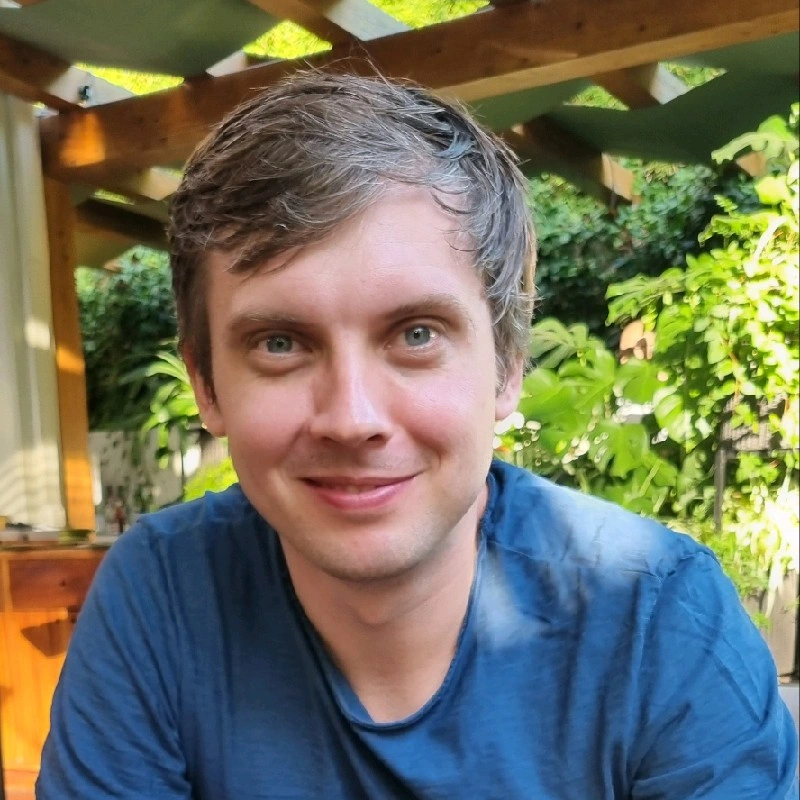
\includegraphics[width=3.5cm]{photo.jpg}}\\
  Zurich, Switzerland / Remote & \\
  Email: \href{mailto:dmitri@manajev.com}{dmitri@manajev.com} & \\
  GitHub: \href{https://github.com/legalaspro}{github.com/legalaspro} & \\
  LinkedIn: \href{https://linkedin.com/in/dmitri-manajev/}{linkedin.com/in/dmitri-manajev} & \\
  Web: \href{https://manajev.com/}{manajev.com} & \\
  \ifswissversion
  \textbf{Swiss C permit} | Estonian & \\
  \fi
\end{tabular*}

%-----------SUMMARY-----------------
\section{Summary}
Robotics and Reinforcement Learning Engineer with 15+ years of software engineering experience, including software architecture, engineering leadership, technical product management, and entrepreneurship.
Currently developing and commissioning ROS~2 software in C++ and Python for autonomous robotic systems, spanning navigation, motion control, systems integration, simulation, imitation learning, and real-robot deployment.
Earlier work includes regulated medical software, cloud infrastructure, mobile and web products, and distributed systems.

% --------SKILLS------------
\section{Skills}
 \resumeSubHeadingListStart
    \resumeSubItem{Robotics Software}
      {ROS~2 and ROS~1, ros2\_control, Nav2, Behavior Trees, MoveIt~2, tf2, URDF/Xacro;
       navigation, motion planning and control, manipulation, systems integration,
       failure recovery, commissioning and hardware--software debugging}
    \resumeSubItem{Robot Learning \& Reinforcement Learning}
      {PPO, SAC, TD3, DDPG; multi-agent RL (MAPPO, HAPPO, MADDPG);
       offline-to-online RL (RLPD); LeRobot policies (ACT, SmolVLA);
       reproducible training/evaluation, sim-to-real and real-robot deployment}
    \resumeSubItem{AI/ML \& Simulation}
      {PyTorch (primary), JAX, TensorFlow, NumPy, OpenCV;
       Gazebo, MuJoCo, Isaac Gym, Unity ML-Agents;
       Gymnasium, PettingZoo, SMACv2, Weights \& Biases, Hugging Face Hub}
    \resumeSubItem{Software Engineering \& Infrastructure}
      {Linux (Ubuntu), Git, Docker, CMake, automated testing,
       CI/CD (GitHub Actions, Jenkins), Ansible, AWS and nginx;
       AI-assisted development workflows (Claude Code, OpenAI Codex)}
    \resumeSubItem{Programming Languages}
      {C++ and Python; additional production experience with JavaScript/TypeScript,
       Swift/Objective-C, Solidity, C\#, and SQL/NoSQL}
    \resumeSubItem{Architecture, Product \& Leadership}
      {Software architecture, engineering-team leadership, technical product management,
       PRDs/specifications, roadmaps/backlogs, Agile delivery and regulated software releases}
 \resumeSubHeadingListEnd

%-----------LANGUAGES-----------------
\section{Languages}
\small English (fluent), German (A2/B1)

%-----------EXPERIENCE-----------------
\section{Experience}
  \resumeSubHeadingListStart
    \resumeSubheading
      {\href{https://hivebotics.tech/}{Hivebotics} \textnormal{\textemdash\ autonomous robotics}}{Remote + on-site, Singapore}
      {Robotics Engineer (Independent Contractor)}{May 2026 -- Present}
      \resumeItemListStart
        \resumeItem{Develop and commission ROS~2 software in C++ and Python for autonomous cleaning robots, covering navigation, manipulation, motion control and systems integration.}
        \resumeItem{Improve real-world reliability through cross-stack debugging, recovery handling, simulation/real-robot validation and field diagnostics.}
        \resumeItem{Supported on-site integration, testing and commissioning in Singapore.}
      \resumeItemListEnd

    \resumeSubheading
      {Manajev AI Labs}{Zurich, CH}
      {Freelance Robotics / AI Software Engineer}{Mar 2026 -- Present}
      \resumeItemListStart
        \resumeItem{\textbf{Analytics company (Switzerland) \textemdash\ robotics simulation research} (Mar -- May 2026): developed PX4/ROS~2 control and simulation prototypes in Gazebo and Unity; established reproducible development and GPU simulation environments.}
        \resumeItem{\textbf{\href{https://app.theconstruct.ai/l/72c786b5/}{The Construct \textemdash\ course author}} (Mar -- May 2026): designed and built a physical-AI robot-arm course covering SO-101/ROS~2 integration, data collection, LeRobot/ACT policy training and edge deployment; \href{https://github.com/legalaspro/so101-ros-physical-ai}{public ROS~2 project and demos}.}
      \resumeItemListEnd

    \resumeSubheading
      {Independent Robotics \& RL R\&D \textnormal{(self-directed)}}{Zurich, CH}
      {Self-directed robotics portfolio and structured RL study}{Dec 2024 -- Feb 2026}
      \resumeItemListStart
        \resumeItem{Built reproducible RL training/evaluation pipelines for multi-agent and continuous-control tasks (Unity ML-Agents, PettingZoo); ran algorithm benchmarks with documented experiment artifacts (\href{https://github.com/legalaspro}{GitHub}).}
        \resumeItem{Implemented ROS~2/C++ control loops for policy deployment; navigation, waypointing, manipulation and sim-to-real on differential-drive/holonomic bases and 5/6-DoF arms, incl. LeRobot imitation learning.}
      \resumeItemListEnd

    \resumeSubheading
      {CryptoApps Manajev}{Zurich, CH}
      {Founder \& Software Engineer}{Aug 2018 -- Dec 2024}
      \resumeItemListStart
        \resumeItem{Designed, built and shipped full-stack decentralized applications on Ethereum and Tron (Solidity, Node.js, Vue.js), incl. smart-contract security analysis and audits.}
        \resumeItem{Built automated transaction-routing systems and execution bots for high-throughput distributed environments; optimized Ethereum/Tron/EOS node infrastructure for latency and cost.}
      \resumeItemListEnd

    % Swissmeda — Role 1
    \resumeSubheading
      {Swissmeda AG}{Zurich, CH}
      {Product \& IT Manager / Software Architect / DevOps}{Nov 2015 -- Jun 2018}
      \resumeItemListStart
        \resumeItem{Led the software engineering team (backlog planning, 1:1s, delivery); authored product specs/PRDs and drove iOS, desktop and backend releases under medical-software regulatory requirements.}
        \resumeItem{Designed and ran AWS cloud infrastructure; migrated the company to GitHub, Jira, Confluence and Linux and standardized CI/CD and release workflows across mobile, desktop and backend.}
        \resumeItem{Architected and shipped the \textbf{smop} iOS app for 3D implant plan review (\href{https://apps.apple.com/us/app/smop/id971741467}{\textbf{App Store}}).}
      \resumeItemListEnd

    % Swissmeda — Role 2 (separate entry)
    % Some parsers have problem parsing 2 job roles for same company
    \resumeSubheading
      {Swissmeda AG}{Zurich, CH}
      {Senior iOS Engineer}{Apr 2014 -- Oct 2015}
      \resumeItemListStart
        \resumeItem{Architected the multi-brand \href{https://apps.apple.com/us/app/smop/id971741467}{\textbf{smop}} iOS app (3D implant plan viewing, slice navigation, case review); automated build/deploy with Fastlane and CocoaPods.}
      \resumeItemListEnd

    \resumeSubheading
        {SpotMe (Shockfish SA)}{Lausanne, CH}
        {Senior Full-Stack Engineer}{Jan 2013 -- Feb 2014}
        \resumeItemListStart
            \resumeItem{Built real-time event features (voting, photo sharing, check-in, surveys, data viz) across backend and mobile web (Node.js, CouchDB, d3.js) for multiple client projects on tight deadlines.}
        \resumeItemListEnd

    \resumeSubheading
      {Life Ideas}{St. Petersburg, RU}
      {Creator / Mobile Software Engineer}{Jan 2012 -- Jan 2013}
      \resumeItemListStart
          \resumeItem{Created \textbf{Instacam}, the first unofficial Instagram client for Windows Phone 7, with a photo-filter engine and 7 social-network integrations; \href{https://www.redmondpie.com/instagram-for-windows-phone-7-is-unofficially-here/}{\textbf{media coverage}} and broad adoption.}
      \resumeItemListEnd

    \resumeSubheading
      {Lanit-Tercom}{St. Petersburg, RU}
      {Intern to Software Engineer}{Jan 2010 -- Dec 2012}
      \resumeItemListStart
          \resumeItem{Developed mobile apps (iOS, WP7, Android), a project-management web app and a WPF/.NET desktop GUI for analytical instruments for outsourcing clients.}
      \resumeItemListEnd

  \resumeSubHeadingListEnd


%-----------EDUCATION-----------------
\section{Education}
  \resumeSubHeadingListStart
    \resumeSubheadingInfo
      {St. Petersburg State University (SPbSU)}{St. Petersburg, Russia}
      {M.Sc.-equivalent Specialist Degree in Software Engineering \& Mathematics}{2007 -- 2012}
      {\textbf{Thesis}: Collaborative recommendation system for tourist attractions.}
  \resumeSubHeadingListEnd


%-----------CERTIFICATIONS \& TRAINING-----------------
\section{Certifications \& Training}
  \resumeSubHeadingListStart
    \resumeCertItem{\href{https://app.theconstruct.ai/accomplishments/verify/RIA34BEEEEF7B59/}{Robotics Developer (Masterclass), The Construct}}{Sep 2025 -- Mar 2026}
    \resumeCertItem{\href{https://www.theconstruct.ai/unitree-g1-humanoid-robotics-certificate-training/}{Humanoid Robotics Certificate, Unitree G1 (Barcelona), The Construct}}{Dec 2025}
    \resumeCertItem{\href{https://www.udacity.com/certificate/e/a3bacae8-bb66-11ed-826d-cbcb7e7fecc7}{Deep Reinforcement Learning (Nanodegree), Udacity}}{Nov 2024 -- May 2025}
    \resumeCertItem{\href{https://www.udacity.com/certificate/e/7d6c9ede-5fc5-11ef-b8e4-0bf0243c348f}{Data Analysis with Pandas \& NumPy, Udacity}}{Sep 2024}
    \resumeCertItem{\href{https://www.udacity.com/certificate/e/6c29da6e-75b7-11ed-b96b-671d91689ee6}{Machine Learning with PyTorch (Nanodegree), Udacity}}{2023}
    \resumeCertItem{\href{https://www.udacity.com/certificate/e/9ff0fd60-75b6-11ed-984e-53126f988a5f}{Full Stack JavaScript Developer (Nanodegree), Udacity}}{2023}
\resumeSubHeadingListEnd


%-------------------------------------------
\end{document}
